Our in-context function estimation model consist of an encoder and two decoders. The encoder and the first decoder can be interpreted as the branch and trunk nets from DeepONets \citet{Lu_2021}. Like \citet{seifner2025zeroshotimputationfoundationinference} we predict the mean and log variance of a gaussian distribution for each data point. \autoref{fig:model} shows our model architecture. We use the Attention is all you need transformer encoder (\citet{vaswani2017attention}) for generating a representation of the input sequence and using this information we employ two decoders to predict the mean and log variance for a specific point in time. When processing unseen data, the input sequence of known context points are first processed by the encoder. Then the decoders are used to predict all points on a grid. We use a grid of 128 points on an interval of $[0,1]$. This means, we run the decoders 128 times with corresponding output time indices. The encoder result is only calculated once. 

\label{impl:model}
	\begin{figure}
		\centering
	\begin{tikzpicture}
	\node at (0,0) (A)  {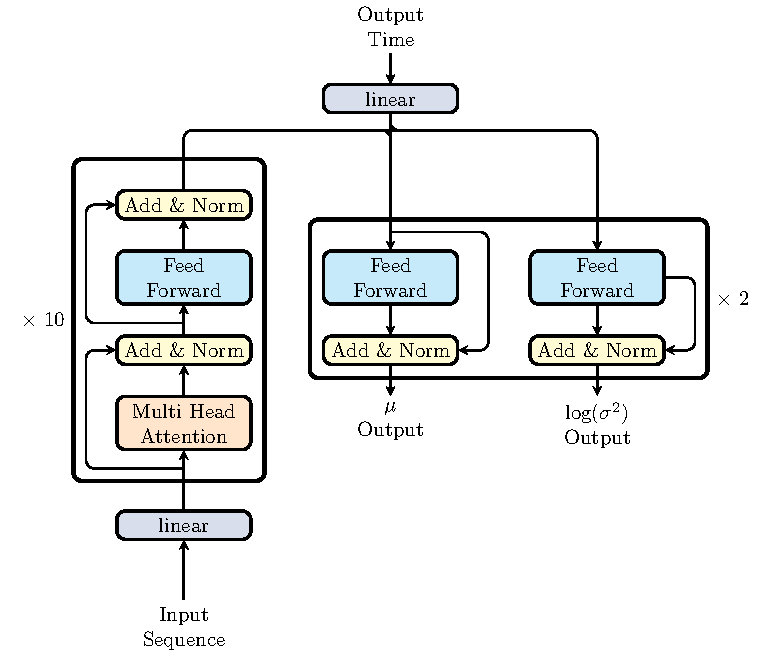
\includegraphics[width=\linewidth]{figures/architecture.pdf}};
	\end{tikzpicture}
	\label{fig:model}
	\caption{In-context function estimation model based on a transformer encoder and feed forward decoders.}
\end{figure}

We normalize values and time indices as part of the model implementation. Like \citet{seifner2025zeroshotimputationfoundationinference} we employ min-max normalization for the input sequence (time indices and values). During training the target sequence is normalized as well and the loss is computed on the normalized data. \autoref{eq:norm} shows the general formula for normalizing data. During training, the min and max values for normalizing both input and target values are determined from the input data. When predicting results we denormalize the mean and standard deviation value. Denormalizing predicted mean values in \autoref{eq:denorm} differs from denormalizing the standard deviation in \autoref{eq:denorm_std}, as only its scale has to be denormalized. Note that \autoref{eq:denorm_std} includes the predicted log variance for completeness.

\begin{align}
x_i &\leftarrow \dfrac{x_i-x_{\text{min}}}{x_{\text{max}}-x_{\text{min}}} \label{eq:norm} \\
\mu &\leftarrow \mu (x_{\text{max}}-x_{\text{min}}) + x_{\text{min}} \label{eq:denorm} \\
\sigma &= \sqrt{e^{\text{log}(\sigma^2)}} x_{\text{max}}-x_{\text{min}} \label{eq:denorm_std} 
\end{align}



